%%%%%%%%%%%%%%%%%%%%%%%%%%%%%%%%%%%%%%%%%%%%%%%%%%%%%%%%%%%%%%%%%%%%%%%%
%                                                                      %
%     File: Thesis_Background.tex                                      %
%     Tex Master: Thesis.tex                                           %
%                                                                      %
%     Author: Andre C. Marta                                           %
%     Last modified :  4 Mar 2024                                      %
%                                                                      %
%%%%%%%%%%%%%%%%%%%%%%%%%%%%%%%%%%%%%%%%%%%%%%%%%%%%%%%%%%%%%%%%%%%%%%%%

\chapter{Background}
\label{chapter:background}

In previous section, the importance of the topic of this thesis was discussed. In this chapter, the background of the topic is further presented where the problema is physically and mathematically define and the theory is explored. The main goal of this chapter is to provide a solid foundation for the reader to understand the problem and the proposed approach.

A key starting point is to define the body, in this case the spacecraft model to be analyzed. The spacecraft is considered a point-mass simulating the desired payload to recover, with a rotor coupling. On Fig. \ref{fig:mode_vehicle}, it is presented a four blade rotor, coupled to the point-mass. The point mass does not play any role rather than be influenced with the gravity field which will pull the vehicle to the ground, and has no dimensions, only mass. On Fig. \ref{fig:mode_vehicle}, the point-mass is represented as a black dot for better visual understanding

On the other hand, the rotor is defined by the blades , which are considered to be rigid, with a blade span, $S_b$, equal for all blades. The rotor has a certain number of blades, Nb, 4 in the case of Fig. \ref{fig:mode_vehicle}. Also, the blades are equally distributed, with the angle between the blades, $\delta\psi$, equal for symmetry reasons.

\begin{figure}[!htb]
    \centering
    \includegraphics[width=7cm]{Figures/background/model_vehicle.png}
    \caption{Vehicle model considered with a four blade rotor}
    \label{fig:mode_vehicle}
\end{figure}

\section{Reference Frames}

For the development of the mathematical model that follows and considering what was present it is important to introduce the reference frames which will define the vehicle’s dynamics. On Fig. \ref{fig:reference_frames} the two principal references are presented: Earth frame, $O^i$, (black axes in Fig. \ref{fig:reference_frames}) and the rotor’s frame $O^r$ (red axes in Fig. \ref{fig:reference_frames}). The Earth frame, $O^i$, is a inertial frame positioned in any point of the Earth surface. It is also called  \textit{Navigation Frame} \cite{soler_fundamentals_2014} once it rotates with Earth and it is very handy when planes to travel from one point to another \cite{soler_fundamentals_2014}. On other hand, the rotor frame, $O^r$, or body frame \cite{soler_fundamentals_2014} is a system axes centered in any point of the symmetry plane of the aircraft. In this case, the $O^r$ is position at the \gls{cg} of the vehicle which is coincident with the point-mass position. The $O^r$ as its $z$-axis aligned, from the \gls{cg}, vertically with the rotor's shaft pointing positively upwards the rotor.

\begin{figure}[!htb]
    \centering
    \includegraphics[width=6cm]{Figures/background/reference_frames.png}
    \caption{Illusttration of the reference frame}
    \label{fig:reference_frames}
\end{figure}

Also there are other theree important reference frames in order to apply \gls{bet} in Fig.\ref{fig:reference_frames}: the blade reference frame (red axes in Fig. \ref{fig:reference_frames}), the element reference frame (green axis in Fig. \ref{fig:reference_frames}) and the 2D aerodynamic reference frame (purple axes in Fig. \ref{fig:reference_frames}). This axes detailed explained further is Sec. \ref{section:bet} and given contest only for \gls{bet}.

Note that, from here on, when a variable or vector is written in any reference frame, it will be denoted by its correspondent superscript, e.g., if a variable or vector, $x$, is written in the rotor frame, it will be denoted by $x^r$.


%%%%%%%%%%%%%%%%%%%%%%%%%%%%%%%%%%%%%%%%%%%%%%%%%%%%%%%%%%%%%%%%%%%%%%%%
\section{Vehicle Dynamics}
\label{section:vehicle_dynamics}

The spacecraft is nevertheless able to translate and rotate in space, meaning that a \gls{6dof} dynamic model is considered. The dynamic model is based on the Newton's second law of motion \cite{soler_fundamentals_2014,vepa_flight_2023}, which states that the acceleration of an object is directly proportional to the net force acting upon the object and inversely proportional to the object. For the translation motion Eq. \ref {eq:force_equation} is used \cite{soler_fundamentals_2014,vepa_flight_2023}.

\begin{equation}
    \mathbf{F}^i = \frac{\mathrm{d}}{\mathrm{d}t} \left( m \mathbf{V} \right)^i
    \label{eq:force_equation}
\end{equation}

\noindent where $\mathbf{F} \in \mathbb{R}^3$ is the external force, $m$ is the mass of the vehicle in \unit{kg}, $\mathbf{V} \in \mathbb{R}^3$ is the vehicle’s linear velocity in \unit{m/s}. 

In terms of the applied forces, once it is considered the recovery of a spacecraft the Earth's gravity force is applied at the point-mass model, meaning no rotation will occur due to gravity. Other important force is the rotor force. So, the to compute the total force, $\mathbf{F}^i \in \mathbb{R}^3$, in \unit{N}, 

\begin{equation}
    \mathbf{F}^i = \mathbf{F}_{gravity}^i + \mathbf{F}_{rotor}^i,
\end{equation}

\noindent where also $\mathbf{F}_{gravity}^i \in \mathbb{R}^3$ and $\mathbf{F}_{rotor}^i \in \mathbb{R}^3$ are in \unit{N}.

Regarding the angular motion, the sum of external moments $\mathbf{M} \in \mathbb{R}^3$, in \unit{N/m}, at the \gls{cg} is equal to the rate of change in angular momentum \cite{soler_fundamentals_2014,vepa_flight_2023},

\begin{equation}
    \mathbf{M}^i = \frac{\mathrm{d}}{\mathrm{d}t} \left( \left[\mathbf{I}\right] \boldsymbol{\omega} \right)^i \Leftrightarrow  \mathbf{M}^r = \frac{\mathrm{d}}{\mathrm{d}t} \left( \left[\mathbf{I}\right] \boldsymbol{\omega} \right)^r + \boldsymbol{\omega} \times \left( \left[\mathbf{I}\right] \boldsymbol{\omega} \right)^r
    \label{eq:momentum_equation}
\end{equation}

\noindent where $\left[\mathbf{I}\right]$, in \unit{kg/m^2}, is the mass inertia tensor. 

From the vehicle dynamics prespective in Eq. \ref{eq:momentum_equation}, the \gls{cd} model, Fig. \ref{fig:rotor_cd}, of the rotor does not change its position inside the rotors's reference frame and any moment generate by the rotor implies also the rotation of the rotor referece frame in Earth's reference frame, $O^i$. When rotated, the angles between the Earth referece frame, $O^i$, and the rotor’s reference frame, $O^r$, are called the Euler angles, and are denoted $\boldsymbol{\Omega}_E \in \mathbb{R}^3$.

\begin{figure}[!htb]
    \centering
    \includegraphics[width=6cm]{Figures/background/rotor_cd.png}
    \caption[Rotor considered as CD, with rotor's reference frame, $O^r$, origin in its center]{Rotor considered as \gls{cd}, with rotor's reference frame, $O^r$, origin in its center}
    \label{fig:rotor_cd}
\end{figure}

Hence, there is a degree of freedom given by the rotor's shaft which means that the rotation of the rotor over $z$-axis of $O^r$ can be decoupled to another equation and, mathematically, the moment applied does not rotate the rotor's reference frame by its on axis.


\subsection{Gravity Force}

The gravitational force acting on the rotor, represented by the vector \(\mathbf{F}_{gravity}^i \in \mathbb{R}^3\) in \unit{N}, can be expressed in the inertial reference frame as a three-dimensional vector. According to \cite{curtis_orbital_2008}, this force can be expressed in vector forma as 

\begin{equation}
    \mathbf{F}_{gravity}^i = 
    \begin{bmatrix}
        0 & 0 & -G \frac{m \cdot M_E}{r^2}
    \end{bmatrix}^T,
\end{equation}  

\noindent where $G$ is the gravitational constant, in \unit{m^3/kg \cdot s^2}, $M_E$ is the Earth's mass, in \unit{kg}, and $r$ represents the distance between the vehicle's center of gravity and the Earth's center of mass, in \unit{m}. This force acts along the radial direction, pointing towards the 
Earth's center, and is responsible for the gravitational attraction governing the vehicle's motion within a central gravitational field. Since\ this work considers a flat Earth, the direction is downwards.


\subsection{Inertia Tensor}

The angular momentum is to angular velocity what linear momentum is to linear velocity. Just as mass quantifies the resistance of an object to changes in its position, the mass inertia tensor, $\left[\mathbf{I}\right]$, measures an object's resistance to changes in its rotational motion. Mathematically, the inertia tensor, $\left[\mathbf{I}\right]$, is a symmetric 3 by 3 matrix 

\begin{equation}
    \left[\mathbf{I}\right]=\left[\begin{array}{c c c}{{I_{x x}}}&{{I_{x y}}}&{{I_{x z}}}\\ {{I_{x y}}}&{{I_{y y}}}&{{I_{y z}}}\\ {{I_{x z}}}&{{I_{y z}}}&{{I_{z z}}}\end{array}\right]
\end{equation}

\noindent where the matrix elements are the moments and products of inertia, about a reference frame $O_{xyz}$, computed as equations \ref{eq:ele_tensor_inertia1} and \ref{eq:ele_tensor_inertia2}

\begin{equation}
    I_{xx} = \smallint  \left( y^2 + z^2 \right) \mathrm{d}m \quad \text{and} \quad I_{yy} = \smallint  \left( x^2 + z^2 \right) \mathrm{d}m \quad \text{and} \quad I_{zz} = \smallint  \left( x^2 + y^2 \right) \mathrm{d}m
    \label{eq:ele_tensor_inertia1}
\end{equation}


\begin{equation}
    I_{xy} = - \smallint  xy \, \mathrm{d}m \quad \text{and} \quad I_{xz} = - \smallint  xz \, \mathrm{d}m \quad \text{and} \quad I_{yz} = - \smallint  yz \, \mathrm{d}m
    \label{eq:ele_tensor_inertia2}
\end{equation}

In this study, the system is considered as a point mass and a rotor which means that only the rotor's mass is accounted into the inertia tensor. The rotor is composed by $N_b$ blades and each blade has $m_b$ mass, which, by simplification, are considered as thin-plates for the inertia tensor calculation. In its principal axes centered in blade's center of mass, a thin-plate with its longer side along $y$-axes (the blade span, $S_b$), its shorter side along $x$-axis (the airfoil chord, $c_a$) and its thickness along $z$-axis (the airfoil thickness, $t_a$). The inertia tensor, $\left[\mathbf{I}\right]'$ of a flate plate in its principal axes is computed as in Eq. \ref{eq:inertia_tensor_principalaxes}

\begin{figure}[!htb]
    \centering
    \includegraphics[width=10cm]{Figures/background/inertia/inertia_scheme.png}
    \caption{Thin-plate position according to the principal axes ($O'$) inside the rotor' and blade's coordinate system, $O^r$ and $O^b$, respectively.}
    \label{fig:Inertia}
\end{figure}

\begin{equation}
    \left[\mathbf{I}\right]' = 
    \begin{bmatrix}
        \frac{1}{12}m_b(S_b^2+t_a^2) & 0 & 0\\
        0 & \frac{1}{12}m_b(c_a^2+t_a^2) & 0\\
        0 & 0 & \frac{1}{12}m_b(S_b^2+c_a^2)\\
    \end{bmatrix}
    \label{eq:inertia_tensor_principalaxes}
\end{equation}

For a rotor with multiple blades with a root distance from the blade to the rotor center, a transformation process must be introduced. Defining $\psi$ as the set azimutal position, the blades separated by an angle of

\begin{equation}
    \delta\psi = \frac{2\pi}{N_b}
\end{equation}

\noindent and, setting one of the blade's reference frame aligned with rotor's referece frame, rotation angle of blade $b=1$ over $z$-axis equals to $\Psi_1 = 0$, introducing the rotation matrix, $\boldsymbol{R}^{ot} \in \mathbb{R}^{3 \times 3}$, and considering the parallel axis theorem the total inertia tensor of the rotor in rotor frame is

\begin{equation}
    \left[\mathbf{I}\right]^r = \sum_{m=1}^{N_b} \boldsymbol{R}_n^{ot}\left[(m-1)\delta\psi\right] \left\{ \left[\mathbf{I}\right]' + m_b \epsilon^2 \boldsymbol{\mathcal{I}} \right\} \boldsymbol{R}_n^{ot}\left[(m-1)\delta\psi\right]^T
\end{equation}

\noindent where $\epsilon$ stands for the distance of the blade's centroid to the rotor’s reference frame, $O^r$, and $\boldsymbol{\mathcal{I}} \in \mathbb{R}^{3 \times 3}$ is an identity matrix.




%%%%%%%%%%%%%%%%%%%%%%%%%%%%%%%%%%%%%%%%%%%%%%%%%%%%%%%%%%%%%%%%%%%%%%%%

\section{Rotor's Dynamics}
\label{section:rotor_dynamics}

For the rotor's dynamics, further considerations shall be made to properly account for the generation of forces acting on the payload's point-mass model and the moments that provide rotational freedom to the rotor's \gls{cd} model, Fig. \ref{fig:rotor_cd}. In reality, the rotor rotates along its shaft, and this motion is crucial for its aerodynamic analysis. The rotational behavior directly influences the aerodynamic loads, which must be accurately modeled to capture the effects on both the rotor and the payload.

One of the primary concerns is the influence of rotational inertia and the torques that develop due to aerodynamic and inertial effects. The equation concerning the rotor’s rotational dynamics over its shaft, can be expressed as

\begin{equation}
    \frac{\mathrm{d}\Omega}{\mathrm{d}t} = \tau_z
    \label{eq:rotation_eq},
\end{equation}

\noindent where $\Omega$ represents the angular acceleration, in \unit{rad/s}, and $\tau_z$ represents the angular momentum along the $z$-axis fo the rotor's reference frame, $O^r$, computed as 
\begin{equation}
    \tau_z = \frac{T}{I_{zz}},
\end{equation}

\noindent with, $T$ is the applied torque, in \unit{N/m}, and $I_{zz}$ is the moment of inertia about the rotor’s principal axis of rotation. in \unit{kg/m^2}.

The goal of this approach is to effectively handle the high rotational velocities characteristic of rotor operation. When the rotor is spinning at high speeds, numerical stability becomes a concern, particularly when integrating the equations of motion \cite{arnold_numerical_2011,press_numerical_2007}. The time-step used in the \gls{ode} solver must be carefully selected to maintain accuracy without introducing excessive computational cost. A finer discretization may be required to capture the rapid variations in forces and moments in high speeds while ensuring the solver remains efficient.

So instead of define a more finer discretization it is considered not only an blade load distribution, but also an azimultal load distribution for each time step which will not affect numerical stability or create difficults when the Eqs. \ref{eq:momentum_equation} and \ref{eq:rotation_eq} are uncoupled.

\subsection{Blade Element Theory (BET)}
\label{section:bet}

\begin{figure}[!htb]
    \centering
    \includegraphics[width=10cm]{Figures/background/bet/blade.png}
    \caption{\gls{bet} model with an highlight blade element in red. The blade reference frame (in blue) and the element reference frame (in green) are shown. Also the $n$-element velocity vector $\mathbf{U}_n$ in element reference frame is shown. Note that here the $z$-axis is not presented, however applying the right-hand rule it is possible to determine that its direction its towrds the reader.}
    \label{fig:blade_bet}
\end{figure}

The \gls{bet} is a simplified model to study the rotor performance \cite{leishman_principles_2006}. With \gls{bet}, it is possible to make predictions about radial and azimuthal aerodynamic load distributions over the rotor disk. Its principel is based in a quasi-2D airfoils blade section which generate the aerodynamic forces and moments that shall be integrated over the blade length. With \gls{bet} methodology is possible to performe a rotor's first designing shape stage in terms of blade geometry.

Figure \ref{fig:blade_bet} presents the basic idea for the \gls{bet} in which it is possible a blade element $n$ (in red) with a width $\mathrm{d}y$ at a distance $y$ from the blade root. The $n$-element is considered as a 2D airfoil under a flow with a velocity $\mathbf{U}_n \in \mathbb{R}^3$, \ta{in element's reference frame, $O^e$},

\begin{equation}
    \mathbf{U}_n^e = 
    \begin{bmatrix}
        U_t \\
        U_r \\
        U_p \\
    \end{bmatrix}
    \label{eq:velocity_vector_in_element}
\end{equation}

\ta{\noindent where $U_t$ is the tangential component of the velocity, $U_r$ is the radial component of the velocity and $U_p$ is the vertical component of the velocity. The radial velocity component, $U_r$, is usually not considered for lift, by the independence principle, but it is considered when computing the drag in forward flight \cite{leishman_principles_2006}. When considering a 2D airfoil discretization of the blade, the radial velocity $U_r$, is not taking into consideration for the 2D analysis. So, the resultant velocity at the blade element $n$ is computed as}

\begin{equation}
    U_n = \sqrt{U_T^2 + U_p^2} \equiv || \mathbf{U}_n^e ||.
    \label{eq:result_vel_norm}
\end{equation}

For each blade element, the general flow and forces applied and the pressure center of the airfoil are presented in figure \ref{fig:element_bet}. All over the blade and azimutal postions this is not a standard configuration for the reference frames, forces and velocities. This influences the way that angles are determined in each element. This is taken into considerantion and the following equations are for all the cases different.

\begin{figure}[!htb]
    \centering
    \includegraphics[width=9cm]{Figures/background/bet/element.png}
    \caption{Blade element with flow enviroment and forces aplied. Note that here the $y$-axis is not presented, however applying the right-hand rule it is possible to determine that its direction its towrds inside the page.}
    \label{fig:element_bet}
\end{figure}

The aerodynamic loads, in the aerodynamic reference frame, $O^a$, are also represented in figure by \ref{fig:element_bet}, where its horizonal compenent (in $X^a$ axis) or drag force, $\mathrm{d}D_n^a$, is computed as

\begin{equation}
    \mathrm{d}D^a_n = \frac{1}{2} \rho c U_n^2 C_d,
    \label{eq:drag_element}
\end{equation}

\noindent while vertical compenent (in $Z^a$ axis) or lift force is computed as

\begin{equation}
    \mathrm{d}L^a_n = \frac{1}{2} \rho c U_n^2 C_l,
    \label{eq:lift_element}
\end{equation}

\noindent where $\rho$ is air density, in \unit{\kg\per\meter^3}, $c$ is the airfoil cord in \unit{\meter} and $C_l$ and $C_l$ are the lift and drag coefficients, respectively, as functions of the angle of attack, $\alpha$, and number of Reynolds, $Re$,

\begin{equation}
    Re = \frac{\rho U_n c}{\mu}
    \label{eq:reynolds_number}
\end{equation}

\noindent where $\mu$ is the dynamic viscosity of the air in \unit{N s/m^2}, meaning that

\begin{equation}
    C_l \equiv C_l(\alpha, Re) \quad \text{and} \quad C_d\equiv C_d(\alpha, Re).
\end{equation}

In section \ref{section:aero_model}, a detailed explanation on how the lift, $C_l$, and drag, $C_d$, coefficients are obtained is presented. Keeping focus on the aerodynamic load, it is possible to construct the elementary aerodynamic force, $d\mathbf{F}^a_n \in \mathbb{R}^3$, in the aerodynamic reference frame, $O^a$, as

\begin{equation}
    d\mathbf{F}^a_n = \begin{bmatrix}
        \mathrm{d}D^a_n \\ 0 \\ \mathrm{d}L^a_n
    \end{bmatrix}
    \label{eq:vector_aero_force}
\end{equation}

In the other words, the vector presented in Eq. \ref{eq:vector_aero_force} is the force vector of each element that shall be writen in Earth-fixed coordinades for the force equation, Eq. \ref{eq:force_equation}. For a simple implementation, the choice stands for computing the aerodynamic reference frame's\ forces, denoted with upscript $^a$, and apply a cicle to compute the rotor's total force , $\mathbf{F}^r_{rotor}$, as as function of all the elementary forces, $\mathrm{d}\mathbf{F}^a_n$, along the blade length and azimutal positions. Then, it is necessary to introduce the rotation matrices between the various reference frames. First from the aerodynamic to element frame, then to blade frame and rotor frame, and final to the Earth-fixed frame. From the blade and to the element reference frame there is only a translation due to the element's position, being $O^e$ with the same orientation that $O^b$,which means that the rotation matrix is the identity matrix, $\boldsymbol{\mathcal{I}}$. So equation \ref{eq:aero_to_blade_force} presents the direct transformation of the elementary aerodynamic force, $d\mathbf{F}^a$, from the aerodynamic reference frame to the blade reference frame.

\begin{equation}
    d\mathbf{F}^b = \boldsymbol{R}^{ot}(\hat{y}, \phi_n) d\mathbf{F}^a
    \label{eq:aero_to_blade_force}
\end{equation}

$\boldsymbol{R}^{ot}(\hat{y}, \phi_n)$ states for the rotation matrix along $y$-axis and the inflow angle for each of the the blade's elemetns, $\phi_n$. The rotation process is described in section \ref{sec:rotation_matrices}. Finally in the rotor reference frame, the elementary force, $d\mathbf{F}^r$, is given by the rotation given by the blades ' azimuthal angle, $\psi_n$, as

\begin{equation}
    d\mathbf{F}^r_n = \boldsymbol{R}^{ot}(\hat{z}, \psi_n) d\mathbf{F}^b
\end{equation}

\noindent or as a sequence of both rotations, $\phi_n$ and $\psi_m$,

\begin{equation}
    d\mathbf{F}^r_n = \boldsymbol{R}^{ot}(\hat{z}, \psi_m) \boldsymbol{R}^{ot}(\hat{y}, \phi_n) d\mathbf{F}^a.
    \label{eq:element_force_rotor_frame}
\end{equation}

In terms of applied torque from the aerodynamic forces to the rotor's center, the elementary torque applied for each element, $d\mathbf{Q}^r_n$, is given by 

\begin{equation}
    d\mathbf{Q}^r_n = \mathbf{r}^r_n \times \left[ \boldsymbol{R}^{ot}(\hat{z}, \psi_m) \boldsymbol{R}^{ot}(\hat{y}, \phi_n) d\mathbf{F}^a \right] 
    \label{eq:element_torque_rotor_frame}
\end{equation}

\noindent where $\mathbf{r}^r_n$ stand for the position vector from the rotor's center to the blade $n$-element. As a simplification of the next formulas, equation  \ref{eq:simplication_rotation_bet} is introduced

\begin{equation}
    \boldsymbol{R}^{ot}(\hat{z}, \psi_m) \boldsymbol{R}^{ot}(\hat{y}, \phi_n) \equiv \underset{a \to r}{\boldsymbol{R}^{ot}}
    \label{eq:simplication_rotation_bet}
\end{equation}

\noindent and then, force expression, \ref{eq:element_force_rotor_frame}, can be rewritten as

\begin{equation}
    d\mathbf{F}^r_n = \underset{a \to r}{\boldsymbol{R}^{ot}} d\mathbf{F}^a.
    \label{eq:element_force_rotor_frame_simplified}
\end{equation}

\noindent and for the torque, \ref{eq:element_torque_rotor_frame}, the same expression can be used

\begin{equation}
    d\mathbf{Q}^r_n = \mathbf{r}^r_n \times \left[ \underset{a \to r}{\boldsymbol{R}^{ot}}  d\mathbf{F}^a \right] 
    \label{eq:element_torque_rotor_frame_simplified}
\end{equation}.

Knowing all the elementary forces and torques, the total force and torque applied to the rotor can be computed by integrating over the blade length between the blade's root, at a distance $\epsilon$, and the blade's tip, at a distance of $L + \epsilon$. For the the $b$-blade's force is given by

\begin{equation}
    \mathbf{F}^r_{m} = \int_\epsilon^{L+\epsilon} d\mathbf{F}^r_n \mathrm{d}y = \int_\epsilon^{L+\epsilon} \underset{a \to r}{\boldsymbol{R}^{ot}}  d\mathbf{F}^a \mathrm{d}y
\end{equation}


\noindent while blade's torque is computed as

\begin{equation}
    \mathbf{Q}^r_{m} = \int_\epsilon^{L+\epsilon} d\mathbf{Q}^r_n  \mathrm{d}y = \int_\epsilon^{L+\epsilon} \mathbf{r} \times \left[ \underset{a \to r}{\boldsymbol{R}^{ot}}  d\mathbf{F}^a \right] \mathrm{d}y
\end{equation}

As a final step, the forces shall be integrated as a function of the rotor's azimutal discretization, $\psi_m$. To achieve this the integration is assumed as an avarage of all of the forces and torques produced for the blade in each of the azimutal sections

\begin{equation}
    \mathbf{F}_{rotor}^r = \frac{N_b }{N_{\psi}} \sum_{m=1}^{N_{\psi}} \mathbf{F}^r_{m} = \frac{N_b }{N_{\psi}} \sum_{m=1}^{N_{\psi}} \int_\epsilon^{L+\epsilon} \underset{a \to r}{\boldsymbol{R}^{ot}}  d\mathbf{F}^a \mathrm{d}y
    \label{eq:total_rotor_force_rotor_frame}
\end{equation}

\begin{equation}
    \mathbf{Q}_{rotor}^r = \frac{N_b }{N_{\psi}} \sum_{m=1}^{N_{\psi}} \mathbf{Q}^r_{m} = \frac{N_b }{N_{\psi}} \sum_{m=1}^{N_{\psi}} \int_\epsilon^{L+\epsilon} \mathbf{r} \times \left[ \underset{a \to r}{\boldsymbol{R}^{ot}}  d\mathbf{F}^a \right] \mathrm{d}y
    \label{eq:total_rotor_torque_rotor_frame}
\end{equation}

Also, in equations \ref{eq:total_rotor_force_rotor_frame} and \ref{eq:total_rotor_torque_rotor_frame}, it is intoduced the term of the number of blades, $N_b$, as the rotor is composed by multiple blades. $\mathbf{F}_{rotor}^r$ and $\mathbf{Q}_{rotor}^r$ expressions models the rotor's aerodynamic behaviour.


\subsection{ Pitch and Incidence Angle, Angle of Attack}

When computing the aerodynamic forces and moments the angle of attack presents a crucial factor for the 2D aerodynamic lift and drag coefficients \ta{are the flow and airfoil angles. In Fig. \ref{fig:phi_angle_pos} and in Fig. \ref{fig:phi_angle_neg} there are presented two general cases of the angles that will be discussed in this section. The diferent between both figures is the airfoil pitch angle, which is positive for Fig. \ref{fig:phi_angle_pos} and negative for Fig. \ref{fig:phi_angle_neg}. Also, about Figs. \ref{fig:phi_angle_pos} and \ref{fig:phi_angle_neg} the flow velocity for the correspondet airfoil is presented in a diferent direction than in Fig. \ref{fig:element_bet}. }

\begin{figure}[!htb]
    \centering
    \begin{minipage}[b]{0.48\textwidth}
        \centering
        \includegraphics[width=6cm]{Figures/background/bet/angles_theta_pos.png}
        \caption{Blade element with flow environment and forces applied. Reference, $O^a$ and $O^e$.}
        \label{fig:phi_angle_pos}
    \end{minipage}
    \hfill
    \begin{minipage}[b]{0.48\textwidth}
        \centering
        \includegraphics[width=6cm]{Figures/background/bet/angles_theta_neg.png}
        \caption{Blade element with flow environment and reference, $O^a$ and $O^e$.}
        \label{fig:phi_angle_neg}
    \end{minipage}
\end{figure}

The velocity component in each blade element, $\mathbf{U}_n^e$, \ta{in the elements} depends on \tc{its radial position due to the rotation motion of the blade} \ta{several factor that are} tac{- this component} is deeply analyzed further in section \ref{sec:velocity_element_bet}. \ta{In this section it is considered that the velocity vector in element's reference frame, $O^e$ was already obtained.}

The angle between the velocity vector and the horizontal plane of the rotor is called the inflow angle, $\phi$ \ta{or $\phi_n$ when considering the $n$-element's inflow angle}. To compute the inflow angle $\phi$, one can introduce an auxiliary unitary vector, $\mathbf{e}_x^e = \begin{bmatrix} -1 & 0 & 0 \end{bmatrix}^\mathrm{T}$, aligned with the $X^e$ axis \tc{and with the velocity vector expressed in the element reference frame}. The cosine of the inflow angle \ta{between} the unitary vector and \ta{the velocity vector, $\mathbf{U}_n^e$ (recall Eq.\ref{eq:velocity_vector_in_element})}, is given by Eq. \ref{eq:cosine_inflow}

\begin{equation}
    \cos \phi = \frac{\mathbf{U}_n^e \cdot \mathbf{e}^e_x}{||\mathbf{U}_n^e|| ||\mathbf{e}_x^e||}
    \label{eq:cosine_inflow}
\end{equation}

\ta{The dot product between the unitary vector, $\mathbf{e}^e_x$, and the velocity vector, $\mathbf{U}_n^e$, is given by}

\begin{equation}
    \mathbf{U}_n^e \cdot \mathbf{e}^e_x = \sum_ {i=1}^3 (\mathbf{U}_n^e)_i \cdot (\mathbf{e}_x^e)_i = U_t
\end{equation}

\noindent \ta{and considering Eq. \ref{eq:unitary_vec_norm}}

\begin{equation}
    || \mathbf{e}^e_x || =  1,
    \label{eq:unitary_vec_norm}
\end{equation}

\noindent \ta{and attending to Eq. \ref{eq:result_vel_norm}, the inflow equation,Eq. \ref{eq:cosine_inflow}, can be simplified as}

\begin{equation}
    \phi_n = \cos^{-1} \left( \frac{U_t}{\sqrt{U_t^2 + U_p^2}}\right)
    \label{eq:final_eq_inflow}
\end{equation}

\ta{Mathematically, the value of Eq. \ref{eq:final_eq_inflow} is in the range of $ 0 \leq \phi_n \leq 180$ \unit{\deg} and in Figs. \ref{fig:phi_angle_pos} and \ref{fig:phi_angle_neg} the positive direction for the angle reference is clockwise, so it is represented a negative inflow angle. So,} the equation \ref{eq:final_eq_inflow} does not take into consideration \tc{both the} \ta{if} $\mathbf{U}_n$ \tc{if it} is upwards or downwards in terms of the $U_p$ component. As seen in \tc{figure \ref{fig:element_bet}} \ta{Figs. \ref{fig:phi_angle_pos} and \ref{fig:phi_angle_neg} }, the inflow angle, $\phi$, is negative but when \ref{eq:cosine_inflow} is used , the angle is positive. For changing this equation \ref{eq:cosine_inflow_corrected} is introduced.

\begin{equation}
    \begin{cases}
        \phi_n = -\cos^{-1} \left( \frac{U_t}{\sqrt{U_t^2 + U_p^2}}\right), \text{ if } U_P <= 0 \\
        \phi_n = \cos^{-1} \left( \frac{U_t}{\sqrt{U_t^2 + U_p^2}}\right), \text{ if } U_P > 0
    \end{cases}
    \label{eq:cosine_inflow_corrected}
\end{equation}

The angle between the airfoil chordline and the horizonal plane of the rotor is called the pitch angle denoted as $\theta$ in figure \ref{fig:element_bet}. The pitch angle, $\theta$, can be defined as collective or cyclic pitch angle. \tc{All of the blade components along the rotor blade have the same collective pitch angle, which means that the pitch changes uniformly throughout the blade. Usually, the pilot regulates this to change the total lift the rotor produces.} \ta{The collective pitch is a control input that changes the pitch angle of all the rotor blades equally and simultaneously, allowing the helicopter to increase or decrease overall lift and thus ascend or descend.} However, when the rotor rotates, the cyclic pitch angle changes \tc{for various blade parts} \ta{for diferent blade azimutal postions over the rotation}.  \tc{By controlling the rotor disc's orientation, this variation enables the aircraft to tilt in a certain direction.} \ta{Controllig the cyclic pitch, the pilot controlls the blade's flapping movement changing the rotation plano and so the rotor's orientation} Asymmetrical lift distribution and directional control are made possible by the cyclic pitch adjustment, which modifies the blade's angle of attack based on its azimuth location. For the present study, \ta{the cyclic pitch is not consider, but the collective pitch is consider} \tc{the pitch angle is set} for each of the blade \tc{'s element} \ta{at its root} and is \tc{the same distribution} \ta{kept constant} for all the blades \tc{that compose the rotor} and does not change over \ta{simulation} time. \ta{In other words, the collective pitch angle is not controlable in this study, but the simulation is able to consider blade twist, being the $n$-element's pitch angle, $\theta_n$, given by Eq.}

\begin{equation}
    \theta_n = \mathcal{T}(\mathbf{r}_n, \theta_0)
\end{equation}

\noindent \ta{$\mathcal{T}$ is a twist distribution function, $\theta_0$ is the collective pitch angle and $\mathbf{r}_n$ the element position}.

The angle of attack, denoted as $\alpha$, is the angle between the airfoil chord line and the relative airflow experienced by the blade element. It is a crucial parameter in determining the aerodynamic forces acting on the blade. The angle of attack depends on both the pitch angle, $\theta$, and the inflow angle, $\phi$, (here, $_n$ Subscripts where omitted though it is considered the $n$-element's pitch and inflow angle) which include \tc{the induced velocity generated by the rotor and the forward motion of the aircraft} all the factors influencing the element's velocity discussed further in Sec. \ref{sec:velocity_element_bet}. 

\ta{To determine the angle of attack considering} \tc{all} \ta{both} pitch angle, $\theta$, and inflow angles, $\phi$, over the blade \tc{length and azimultal distribution, equation} elements, \ta{Figs. \ref{fig:ang-111}-\ref{fig:ang-444} present the three case that shal be considered. It is important to note that in all figures, that the inflow angle is always negative, up to -180 \unit{\deg} or equal to zero, $\phi \leq 0$. This range consideres some different considerantions regarding the type of motion under which the rotor is. However, once it is always considered that the vehicle is in a descent motion the $\phi > 0$ will never be considered. For each case, some considerations can be added:}

\begin{itemize}
    \item \ta{\textbf{Case 1} (Fig.~\ref{fig:ang-111}): The rotor is in axial descent motion and has angular velocity, possibly with forward motion. The angle of attack in this case is given by ($\theta > 0$ and $\phi < 0 \implies \alpha > 0$):}
    \begin{equation}
        \alpha = \theta - \phi
    \end{equation}
    
    \item \ta{\textbf{Case 2} (Fig.~\ref{fig:ang-222}): Similar to \textbf{Case 1}, however, the negative pitch angle is significant. To compute the angle of attack ($\theta < 0$ and $\phi < 0$, but $\theta > \phi \implies \alpha > 0$):}
    \begin{equation}
        \alpha = -(\phi - \theta) = \theta - \phi
    \end{equation}
    
    \item \ta{\textbf{Case 3} (Fig.~\ref{fig:ang-333}): In this case, the inflow angle is greater than the pitch angle, generating a negative angle of attack. This case may occur near the blade tip, where the tangential velocity $U_t$ is greater than the vertical velocity $U_P$.To compute the angle of attack ($\theta < 0$ and $\phi < 0$, but $\phi > \theta \implies \alpha > 0$):}
    \begin{equation}
        \alpha = \theta - \phi
    \end{equation}

    \item \ta{\textbf{Case 4} (Fig.~\ref{fig:ang-444}): From the schematic, the inflow angle is larger than $-90^\circ$, which means the blade element is in a reverse flow regime. This typically occurs on the retreating side of the rotor during forward flight.To compute the angle of attack ($\phi < -90$ \unit{deg}):}
    \begin{equation}
        \alpha = \theta - \phi \text{, if } \theta > 0
    \end{equation}
    \ta{or}
    \begin{equation}
        \alpha = \phi - \theta \text{, if } \theta > 0
    \end{equation}
    
\end{itemize}

\begin{figure}[!htb]
    \centering
    \begin{minipage}[b]{0.48\textwidth}
        \centering
        \includegraphics[width=4cm]{Figures/background/bet/angles-3.png}
        \caption[Angles case 1]{Angles \textbf{case 1}}
        \label{fig:ang-111}
    \end{minipage}
    \hfill
    \begin{minipage}[b]{0.48\textwidth}
        \centering
        \includegraphics[width=4cm]{Figures/background/bet/angles-1.png}
        \caption[Angles case 2]{Angles \textbf{case 2}}
        \label{fig:ang-222}
    \end{minipage}
\end{figure}
\begin{figure}[!htb]
    \begin{minipage}[b]{0.48\textwidth}
        \centering
        \includegraphics[width=4cm]{Figures/background/bet/angles-2.png}
        \caption[Angles case 3] {Angles \textbf{case 3}}
        \label{fig:ang-333}
    \end{minipage}
    \hfill
    \begin{minipage}[b]{0.48\textwidth}
        \centering
        \includegraphics[width=4cm]{Figures/background/bet/angles-4.png}
        \caption[Angles case 4] {Angles \textbf{case 4}}
        \label{fig:ang-444}
    \end{minipage}
\end{figure}


\section{Velocity Vector in Element's Reference Frame}
\label{sec:velocity_element_bet}

\ta{As previous presented, to compute the elementary drag, Eq. \ref{eq:drag_element}, and elementary lift, Eq. \ref{eq:lift_element}, for each blade element, the velocity vector in element's reference frame, $\mathrm{U}_n^e$, plays a major role to dimensionalize the lift, $C_l$, and drag, $C_d$, coefficents. In this section, the main goal is to analyse how the velocity vector is computed and what are the main factors that influence its magnitude and direction.}

\ta{Due to the vehicle dynamics there are two factors: the linear velocity of the point-mass model and the angular velocity of the vehicle,  around its center of mass, coincident with e the point mass model. The linear velocity of the point-mass model, $\mathbf{V}$, is computed considering Eq. \ref{eq:force_equation} and its resultant vector written in the elements reference frame, $\mathbf{V}^e$, as in Eq. \ref{eq:line_vec_element_frame}}

\begin{equation}
    \ta{\mathbf{V}^e = \underset{i \to e}{\boldsymbol{R}^{ot}} \mathbf{V}^i.}
    \label{eq:line_vec_element_frame}
\end{equation}

\ta{\noindent where $\underset{i \to e}{\boldsymbol{R}^{ot}}$ is the rotation matrix from the inertial frame to the element reference frame. For instance, the angular velocity of the vehicle, $\boldsymbol{\omega}$, influence should be considered in the velocity vector computation. The linear component from the vehicle’s angular velocity, $\mathbf{V}^e_\omega$, is computed as in Eq. \ref{eq:line_ang_vec_element_frame}}

\begin{equation}
    \ta{\mathbf{V}^e_\omega = \mathbf{r}^e  \boldsymbol{\omega}^e.}
    \label{eq:line_ang_vec_element_frame}
\end{equation}

\ta{\noindent where, $\mathbf{r}^e$ is the position vector of the element with respect to the center of mass, and $\boldsymbol{\omega}^e$ is the vehicle's angular velocity.}

\ta{Another factor that influences the velocity vector is rotor's angular velocity, $\Omega$. Its linear component can be computed in the element reference frame as in Eq. \ref{eq:rotor_ang_vel_element},}

\begin{equation}
    \ta{V^e_{\Omega} = \mathbf{r}^e \Omega}
    \label{eq:rotor_ang_vel_element}
\end{equation}

\ta{Finally, it is necessary to also consider the rotor’s induced velocity, $\mathbf{v}_i$. The induced velocity is a result of the rotor’s interaction with the surrounding air and is further detailed in Sec. \ref{sec:induced_Velocity}. However, the resultant velocity vector in element $n$ on any blade is computed as Eq. \ref{eq:element_full_velocity}}

\begin{equation}
    \ta{\mathbf{V}_{n}^e = \mathbf{V}^e + \mathbf{V}^e_\omega + V^e_{\Omega} + \mathbf{v}_i^e}
    \label{eq:element_full_velocity}
\end{equation}

\subsection{Induced Velocity}
\label{sec:induced_Velocity}


\section{Rotation matrices}
\label{sec:rotation_matrices}

Considering any inertial reference frame $O(\hat{x},\hat{y},\hat{z})$ and a rotated reference frame $O'(\hat{x}',\hat{y}',\hat{z}')$, the Euler angles, $\boldsymbol{\Omega}_E$ that the define the rotation of $O'$ related to $O$ is presented in figure \ref{fig:rotation_frames_img}

\begin{figure}[!htb]
    \centering
    \includegraphics[width=6cm]{Figures/background/rotation_matrices/rotation_frames.png}
    \caption{Reference frame rotation Euler angles, adapted from \cite{schwab_how_2006}}
    \label{fig:rotation_frames_img}
\end{figure}

The following expressions, presented in equations \ref{eq:rotatio_zz}, \ref{eq:rotatio_yy} and \ref{eq:rotatio_xx}, define the rotation matrices of a rotation over the each of the reference axis $\hat{Z}$, $\hat{Y}$ and $\hat{X}-$axis. For the rotation matrices, it is used a simplified nomenclature where $c_{\delta_{*}}$ are $s_{\delta_{*}}$ are cosine and sine functions of the angle $\delta_{*}$. The total rotation matrix, considering the Tailt-Bryan Convention is

\begin{equation}
    {R o t({\hat{z}},\delta_1)}={\left[\begin{array}{l l l}{1}&{0}&{0}\\ {0}&{c_{\delta_1}}&{-s_{\delta_1}}\\ {0}&{s_{\delta_1}}&{c_{\delta_1}}\end{array}\right]}
    \label{eq:rotatio_zz}
\end{equation}

\begin{equation}
    Rot(\hat{y},\delta_2)=\left[\begin{array}{c c c}{{c_{\delta_2}}}&{{0}}&{{s_{\delta_2}}}\\ {{0}}&{{1}}&{{0}}\\ {{-s_{\delta_2}}}&{{0}}&{{c_{\delta_2}}}\end{array}\right]
    \label{eq:rotatio_yy}
\end{equation}

\begin{equation}
    Rot({\hat{x}},{\delta_3})={\left[\begin{array}{l l l}{{{c}_{\delta_3}}}&{{-{s}_{\delta_3}}}&{{0}}\\ {{{s}_{\delta_3}}}&{{{c}_{\delta_3}}}&{{0}}\\ {{0}}&{{0}}&{{1}}\end{array}\right]}
        \label{eq:rotatio_xx} 
\end{equation}


After defining expressions \ref{eq:rotatio_zz}, \ref{eq:rotatio_yy} and \ref{eq:rotatio_xx}, the rotation matrix between the aerodynamic reference frame adn the rotor reference frame can be computed as

\begin{equation}
    \boldsymbol{R}^{ot}_{a \to r} = \boldsymbol{R}^{ot}(\hat{z}, \psi_m) \boldsymbol{R}^{ot}(\hat{y}, \phi_n) =
    \begin{bmatrix}
    c_{\phi_n} & 0 & s_{\phi_n} \\
    s_{\psi_m}s_{\phi_n} & c_{\psi_m} & -s_{\psi_m}c_{\phi_n} \\
    -c_{\psi_m}s_{\phi_n} & s_{\psi_m} & c_{\psi_m}c_{\phi_n}
    \end{bmatrix}    
    \label{eq:rotatio_aero_rotor}
\end{equation}


%%%%%%%%%%%%%%%%%%%%%%%%%%%%%%%%%%%%%%%%%%%%%%%%%%%%%%%%%%%%%%%%%%%%%%%

\section{2D Aerodynamic Model}
\label{section:aero_model}

As seen in section \ref{section:bet}, the \gls{bet} is a model based on the sum of the contributions of elementary 2D airfoil sections .Then its crucial for its implementation a computational method to obtain the drag, $C_d (\alpha, Re) $, and  lift, $C_l (\alpha, Re)$, coefficients for 2D airfoils, in equations \ref{eq:drag_element} and \ref{eq:lift_element}.

Also \gls{bet} has critical consideration rather the number of elements used to define a blade. The higher the number of elements and azimutal discretization, the higher the number of calculations needed to be perform a rotor analysis. \tc{This means that for a time-dependent model as a free-fall considered in this work, more critical it is, in term of computational time, to perform any simulation.} So a fast model should be considered.

For choosing an airfoil analysis, one must consider the rotor dynamics. In this study, the rotor is under the phenomena of autorotation which has its displacement mainly in descent direction, then some considerations should be made about the angles of attack. On blade's root, the angular velocity is smaller when compared to the blade's tip. Meaning, the inflow angle is mainly composed by a vertical component rather than a horizontal component. So, a wider range of angles of attack should be considered. Also, if it is considered a pure vertical descent mode and small rotor angular velocity, the angles of attack will certainly be near 90 \unit{\deg} meaning that the rotor will work on a stall mode. A reference to the pitch angle, $\theta$, and the blade twist should be made, however for thin airfoils it is known that for angles near 20 $\sim$ 30 \unit{\deg}, depending on thickness and camber, the airfoils starts to operate as a flate plate on stall mode, with completely separate boundary layers. Lastly, concerning the rotor dynamics, once it is considered the horizontal translation of the vehicle, there will exists a reverse flow region where the angles of attack are expected to be higher than 90$^{\circ}$.

The other input concerning the 2D aerodynamic model for $C_l$ and $C_d$ is the Reynolds number, $Re$, computed as presented in Eq. \ref{eq:reynolds_number}. The Reynolds number is directly proportional to two variables that will change with altitude: density, $\rho$, and dynamic viscosity, $\mu$; these variables are computed in the domain of the atmospheric model that is further presented in section \ref{section:atmosphere_model} it will be shown that for the altitudes considered in this work, the Reynolds number is expected to change. Also the velocity component at each section, $||\mathbf{U}^a_n||$, will have diferent values due to the rotor's angular velocity, $\Omega$, and the and vehicle velocity vector, $\mathbf{V}$, changes, and it is also expected to vary, in this case from 0 \unit{m/s}, when the rotor starts, to a defined value when it achieves the phenomena of autorotation.

So, for both angle of attack, $\alpha$, and Reynolds number, $Re$, a range of values should be defined. For the angle of attack, the aerodynamic model should be able to perform calculations for values ranging 

\begin{equation}
    \alpha \in [-180, 180] \unit{\deg},
\end{equation}

and for Reynolds numbers

\begin{equation}
    Re \in [10^3, 10^7].
\end{equation}

\subsection{AERODAS}
\label{sec:aerodas}

Spera (2008) \cite{spera_models_2008} developed an aerodynamic model  maned AERODAS, for to predict lift and drag coefficients for stallel and unstalled airfoils. \tc{The development of horizontal-axis wind turbines is described as a result} \ta{The model was established during the development of horizontal-axis wind turbine as a result} of a Department of Energy-sponsored and NASA-led federal effort that ran from 1973 to 1995. This study develops an empirical model for airfoil lift and drag by fitting test data with algebraic equations, rather than using aerodynamic theory. It includes a wide range of conditions such as different airfoils, Reynolds numbers, and angles of attack, and also models circular cylinders and thin plates.  Unlike previous models, it uses empirical equations derived from actual airfoil behavior at high angles of attack in the post-stall regime, rather than assuming flat plate behavior. Key improvements include expanding the test data set to cover more airfoils and configurations.

The model also considers airfoil thickness in addition to aspect ratio and angle of attack. Its accuracy is evaluated by calculating the mean and standard deviation of the lift and drag data across various airfoils. Finally, the model is applied in Blade Element Momentum (BEM) analysis to predict wind turbine power and fan performance, and its results are compared with measured data to evaluate its effectiveness.

Going deeper into the mathematical prespective, the AERODAS model main goal is to calculate the lift, $C_l$, and drag, $C_d$, curves as function of angle of attack, $\alpha$, Fig. \ref{fig:aerodas_cl_model} and Fig. \ref{fig:aerodas_cd_model} presents the considered curves and highlight the major considerations about the model. In \cite{spera_models_2008}, the main equations for the model are presented in Tab. \ref{tab:aerodas_key_equation}. The key point of AERODAS model is separate the lift and drag curve with equations for pre-stall and post stall regimes.

\begin{figure}[!htb]
	\centering
	\begin{minipage}{0.45\textwidth}
		\centering
		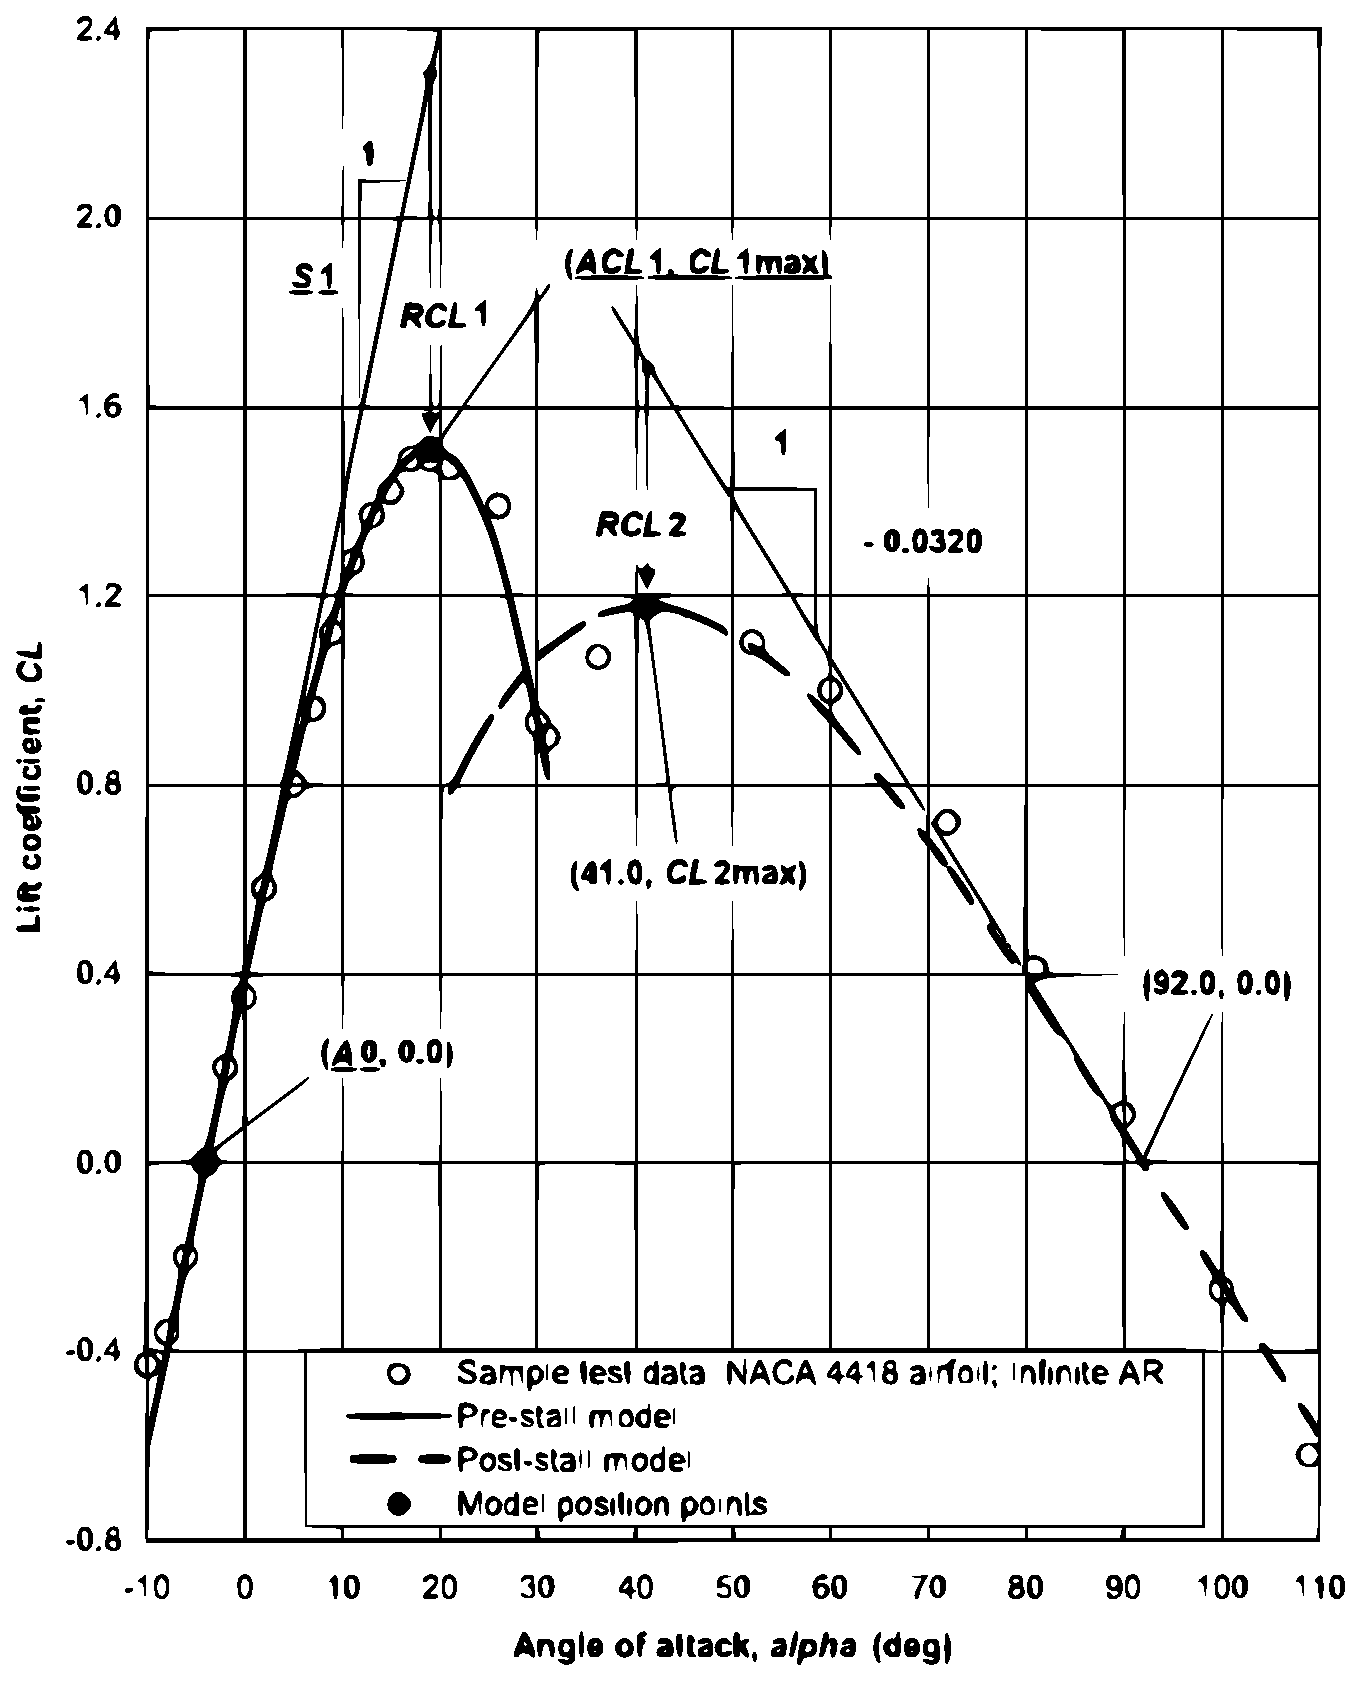
\includegraphics[height=7cm]{Figures/background/aero/liftmodel_aerodas.eps}
		\caption{AERODAS model for lift coefficient, from \cite{spera_models_2008}}
		\label{fig:aerodas_cl_model}
	\end{minipage}
	\hfill
    \begin{minipage}{0.45\textwidth}
		\centering
		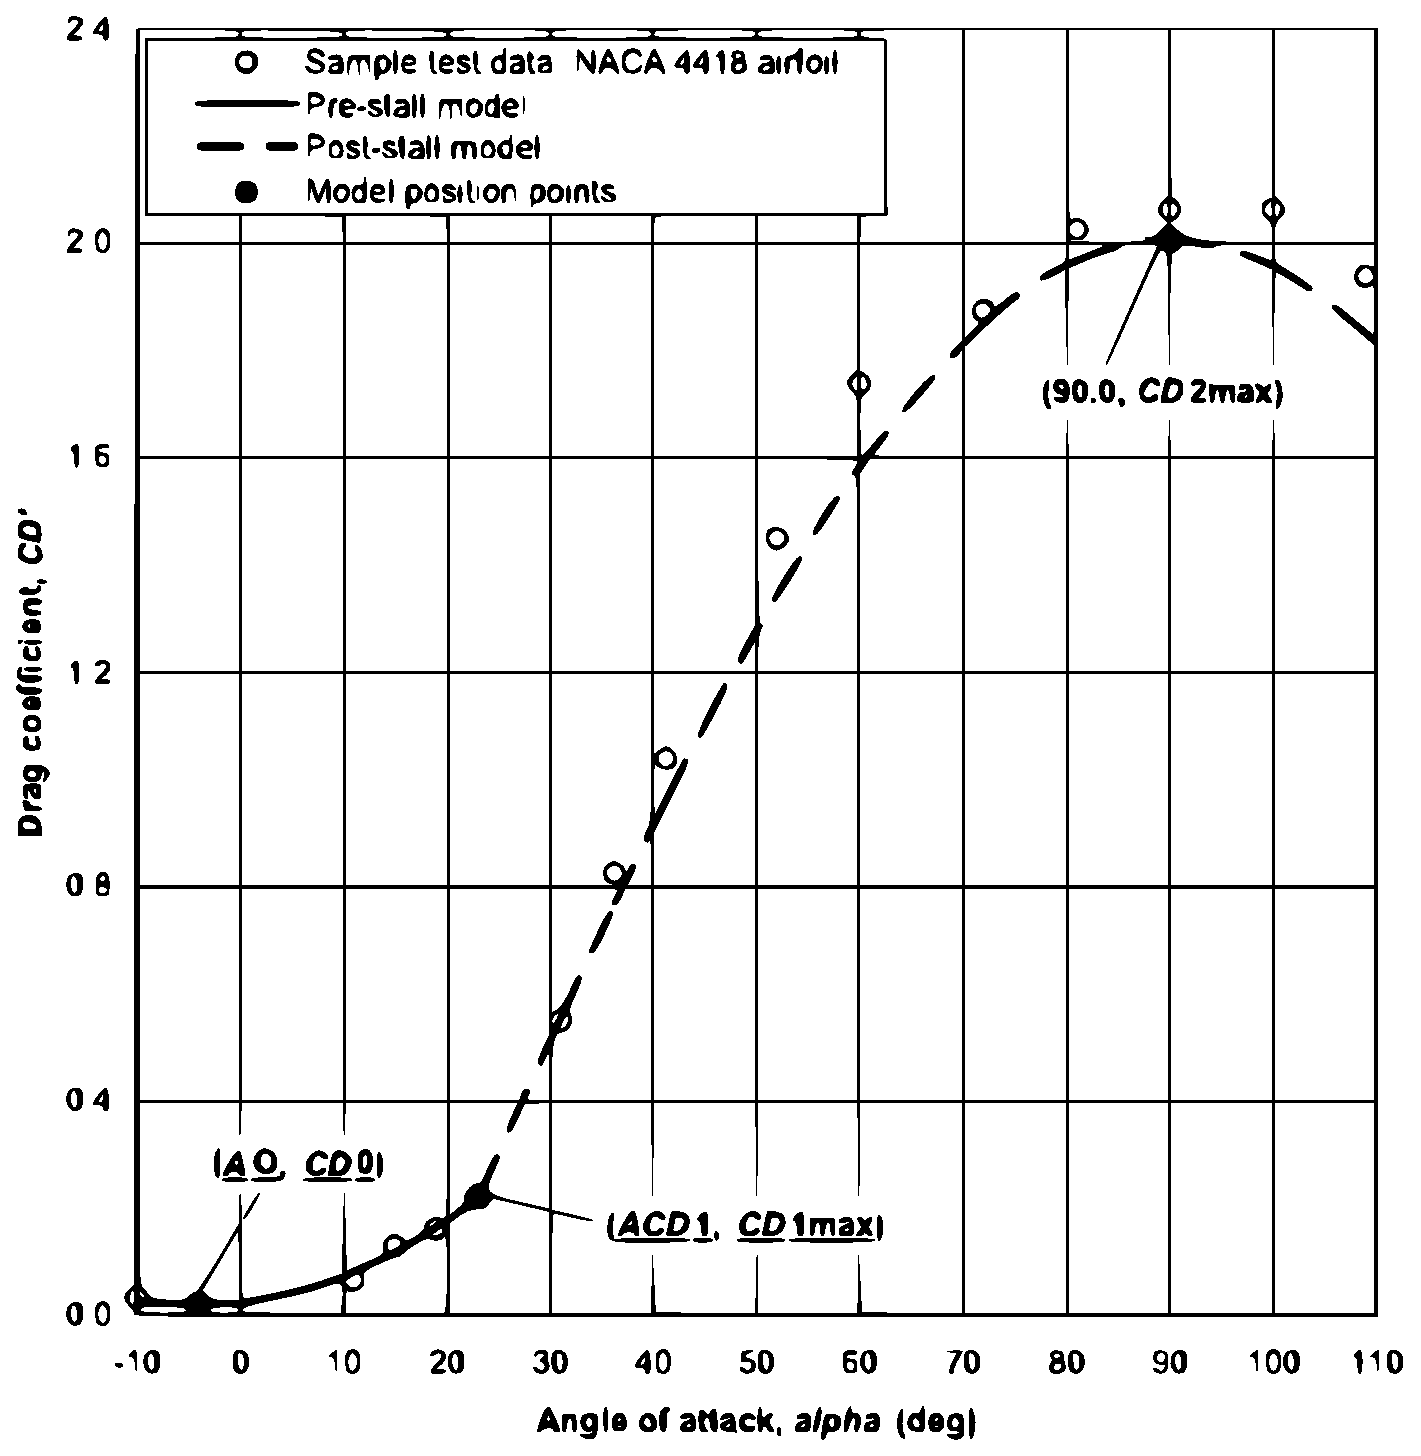
\includegraphics[height=7cm]{Figures/background/aero/dragmodel_aerodas.eps}
		\caption{AERODAS model for drag coefficient, from \cite{spera_models_2008}}
		\label{fig:aerodas_cd_model}
	\end{minipage}
\end{figure}

\begin{table}[!htb]
    \centering
    \renewcommand{\arraystretch}{2.5} % Aumenta o espaço entre as linhas
    \footnotesize % Reduz o tamanho da fonte (use \footnotesize ou \scriptsize se quiser menor ainda)
    \begin{tabular}{llll}
        \hline
        Mode                        & Coefficient                                     & Condition                                   & Equation                                                                                                                    \\ \hline
        \multirow{4}{*}{Pre-stall}  & \multicolumn{1}{c}{\multirow{2}{*}{Lift $CL1$}} & $\alpha \geq A0$                            & $C L1=S1\cdot\left(\alpha-A0\right)-R C L1\left(\frac{\alpha-A0}{A C L1-A0}\right)^{N1}$                                    \\
                                    & \multicolumn{1}{c}{}                            & $\alpha < A0$                               & $CL1=S1\cdot(\alpha-A0)+R C L1\left(\frac{A0-\alpha}{A C L1-A0}\right)^{N1}$                                                \\ \cline{2-4} 
                                    & \multirow{2}{*}{Drag $CD1$}                     & $(2 A0 - ACD1) \leq \alpha \leq ACD1$       & $C D1=C D0+\left(C D1\operatorname*{max}-C D0\right)\left({\frac{\alpha-A0}{A C D1-A0}}\right)^{M}$                         \\
                                    &                                                 & $\alpha < (2 A0 - ACD1)$ or $\alpha > ACD1$ & $CD1=0$                                                                                                                     \\ \hline
        \multirow{7}{*}{Post-stall} & \multicolumn{1}{c}{\multirow{4}{*}{Lift $CL2$}} & $0 < \alpha < ACL1$                         & $CL2=0$                                                                                                                     \\
                                    & \multicolumn{1}{c}{}                            & $ACL1 \leq \alpha \leq 92^{\circ}$          & $CL2=-0.032\left(\alpha-92.0\right) - RCL2\cdot\left({\frac{92.0-\alpha}{51.0}}\right)^{N2}$                                \\
                                    & \multicolumn{1}{c}{}                            & $\alpha > 92^{\circ}$                       & $CL2=-0.032\left(\alpha-92.0\right) + RCL2 \cdot \left(\frac{\alpha-92.0}{51.0}\right)^{N2}$                                \\
                                    & \multicolumn{1}{c}{}                            & $\alpha < 0$                                & $CL2[\alpha] = - CL2[-\alpha + 2 \cdot A0]$                                                                                 \\ \cline{2-4} 
                                    & \multirow{3}{*}{Drag $CD2$}                     & $(2A0-ACL1) \leq \alpha \leq ACL1$          & $CD2 = 0$                                                                                                                   \\
                                    &                                                 & $\alpha \geq ACD1$                          & $CD2 = CD1_{max}+\left( CD2_{max} - CD1_{max}\right) \cdot \sin\left({\frac{\alpha-A C D1}{90.0-A C D1}} \cdot 90\right)$ \\
                                    &                                                 & $\alpha \leq (2A0 - ACD1)$                  & $CD2\big[ \alpha \big] = CD2 \big[- \alpha + A0\big]$                                                                       \\ \hline
        \end{tabular}
    \caption{AERODAS model main equations \cite{spera_models_2008}}
    \label{tab:aerodas_key_equation}
\end{table}

\subsubsection{Pre-Stall Maximum Lift and Drag}

For lift it is defined mathematical expressions for pre-stall, $CL1$, considering \cite{spera_models_2008} uses a proposed model by Viterna, where it consideres a linear variation for the lift coefficient, $S1$, and while $\alpha$ increases approaching the stall angle $ACL1$, the function uses a reduction from extension of linear segment of lift curve to $CL1max$ (maxima $C_l$ value, before stall), $RCL1$,

\begin{equation}
    RCL1 = S1 \cdot (ACL1 - A0) - CL1max
\end{equation}

\noindent and exponent defining shape of lift curve at $ACL1max$, $N1$,

\begin{equation}
    N1 = 1 + \frac{CL1max}{RCL1} 
\end{equation}

In post-stall regime, the lift curve, $CL2$, is modeled by an equation of the same shape as in the pre-stall regime, but with a reversed slope. In this case, the reduction from extension of linear segment of lift curve to $CL2max$

\begin{equation}
    RCL2 = 1.632- CL2max
\end{equation}

\noindent and exponent defining shape of lift curve at $CL2_{max}$, $N1$,

\begin{equation}
    N2 = 1 + \frac{CL2}{RCL2}
\end{equation}

For drag coefficient, its behavior is usually defined considering a quadatic expression \cite{spera_models_2008}. So, AEDODAS model uses 

\begin{equation}
    M = 2
\end{equation}

\subsubsection{Post-Stall Maximum Lift and Drag}

The main goal of AERODAS is to compute the post-stall coefficients of which there is no available experimental data. So to extrapolate data, AERODAS uses two parameteres defining the maximum lift, $CL2max$, and drag, $CD2max$, to compute post-stall curves. To accomplish this goal \cite{spera_models_2008} considers that this coefficients are functions of thickness-to-chord ratio, $t/c$ , and its aspect ratio, $AR$.

\begin{equation}
    CL2max = F1  \left[ t/c \right] \cdot F2 \left[ AR \right] \quad \text{and} \quad CD2max= G1 \left[ t/c \right] \cdot G2 \left[ AR \right]
\end{equation}

For lift coefficient, empirical equations developed follows:

\begin{equation}
    F1=1.190\cdot\left[1.0-\left(t/c\right)^{2}\right] \quad \text{and} \quad F2= 0.65 + 0.35\,\mathrm{exp}\left[-\left(9.0\slash{A}R\right)^{2.3}\right]
\end{equation}

For instance, the empirical equations for maximum drag are

\begin{equation}
    G_1 = 2.300\cdot\,\mathrm{exp}\left\{-\left[0.65\left(\frac{t}{c}\right)\right]^{0.90}\right\} \quad \text{and} \quad G_2 = 0.52 + 0.48\,\mathrm{exp}\left[-\left(\frac{6.5}{A R}\right)^{1.1}\right]
\end{equation}

\subsubsection{Lift and Drag Model Configurations}

Once the model considers coefficients equations in the pre-stall and post-stall regimes separately, it is necessary to select the correct one. This consideration is necessary since for $\alpha \geq ACL1$ (post-stall regime) theres is an overlap between the $CL1$ and $CL2$. For $\alpha < ACL1$ (pre-stall regime), $CL2$ is consider 0, then $CL1$ is the correct expression, for the pre-stall regime.

If $\alpha \geq A0$

\begin{equation}
    C L=\operatorname*{max}(CL1, CL2)
    \label{eq:model alpha a0 greater}    
\end{equation}

If $\alpha \leq A0$

\begin{equation}
    CL = \operatorname*{min}(CL1 , CL2) \quad \text{and} \quad CD = \operatorname*{max}(CD1, CD2)
    \label{eq:model alpha a0 lower}
\end{equation}

\subsection{Neuralfoil Dataset}

This last two definitions \ref{eq:model alpha a0 greater} and \ref{eq:model alpha a0 lower} conclude the computations for lift and drag coefficients as functions of a different set of parameters. This methodology is computationally fast but needs another consideration. For each Reynolds numbers, the $C_l$ vs $\alpha$ and $C_d$ vs $\alpha$ are modelled throw AERODAS with different parameters. So, and considering the range of angles of attack, $\alpha$, and Reynolds numbers, $Re$, it is needed to create a dataset with $C_l$ and $C_d$ curves data for differente $Re$ that shall be process in order to use AERODAS.

In this sense, to lead with this NeuralFoil \cite{sharpe_neuralfoil_nodate} presents a simple solution under the Aerosandbox package \cite{sharpe_aerosandbox_nodate,sharpe_accelerating_nodate}. NeuralFoil is a neural-network based model for 2D airfoils, which is able to predict the drag and lift coefficients for a wide range of airfoils, Reynolds and Mach numbers, and angles of attack. This model is based on a set neural-networks pre-trained with XFOIL meaning that the model is able to predict the drag and lift coefficients inside the scope where XFOIL presents not only numeric convergency but also physical convergency. 

An output parameter from the NeuralFoil (and from any neural-network) is the confidence level of the ouput. This parameter is presented in figure figure \ref{fig:neuralfoil_confidence}, where the black region is the range where the model is able to predict the drag and lift coefficients with a confidence level of 95\%. NeuralFoil \cite{sharpe_neuralfoil_nodate} is a fast and reliable model to predict the drag and lift coefficients for 2D airfoils inside the black region in figure \ref{fig:neuralfoil_confidence}.

\begin{figure}[!htb]
    \centering
    \includegraphics[width=8cm]{Figures/background/aero/NeuralFoil_Confidence_2D_black.png}
    \caption{NeuralFoil confidence level for NACA 0012 airfoil for Reyndols number from $10^3$ to $10^9$}
    \label{fig:neuralfoil_confidence}
\end{figure}

Analysing the figure \ref{fig:neuralfoil_confidence}, it is possible to state some key aspects of the NeuralFoil model:

\begin{enumerate}
    \item As expected NeuralFoil is limited to the angles of attack where XFOIL presents physical convergency - before the the stall angle. This values presents a symmetric result due to the fact that airfoil is also symmetric (without camber).
    
    \item For the ultra low $Re$, below $~ 10^3$, the model is not able to predict the drag and lift coefficients with a confidence level. In this $Re$ interval, the XFOIL is not able to predict the need coefficients once the flow is completely different. At $Re ~ 10^3$ there is an absence of separation bubble as  concluded by Alam er al. (2010) \cite{alam_ultra-low_2010}. Not having a separation bubble the flow keeps laminar for a long longitudinal distance delaying the transition, so no stall occurs, being the maximum coefficients determined at $\alpha \approx 45$ \unit{\deg}
    
    \item At $Re = 10^5 \approx 10^6$, the stall angle varies over the $Re$ interval, meaning it is important to make further consideration for the angles of attack after the stall occurs. After the the stall occurring XFOIL is not able to detemine \tc{the transient phenomena of the flow once it is build based on a panel methos which does not have capabilities to perform an airfoil analysis with time-varient lift and drag coefficients} \ta{the erodynamic coeeficients and it is where AERODAS is capable of work , modeling $C_l$ and $C_d$ with NeuralFoil confidence data}.

\end{enumerate}

\begin{figure}[!htb]
	\centering
	\begin{minipage}{0.3\textwidth}
		\centering
		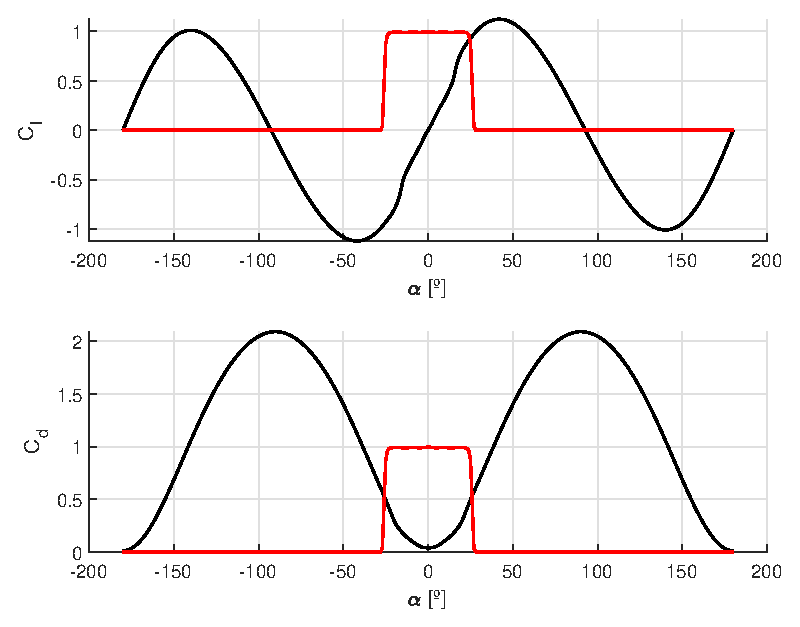
\includegraphics[width=\textwidth]{Figures/background/aero/aero_model_1e4.eps}
		\caption[NACA 0012 airfoil aerodynamic coefficients for $Re=10^4$ determined with Neural foil with confidence level]{NACA 0012 airfoil aerodynamic coefficients (in black) for $Re=10^4$ determined with Neural foil with confidence leve (in red)}
		\label{fig:aero_model_1e4}
	\end{minipage}
	\hfill
	\begin{minipage}{0.3\textwidth}
		\centering
		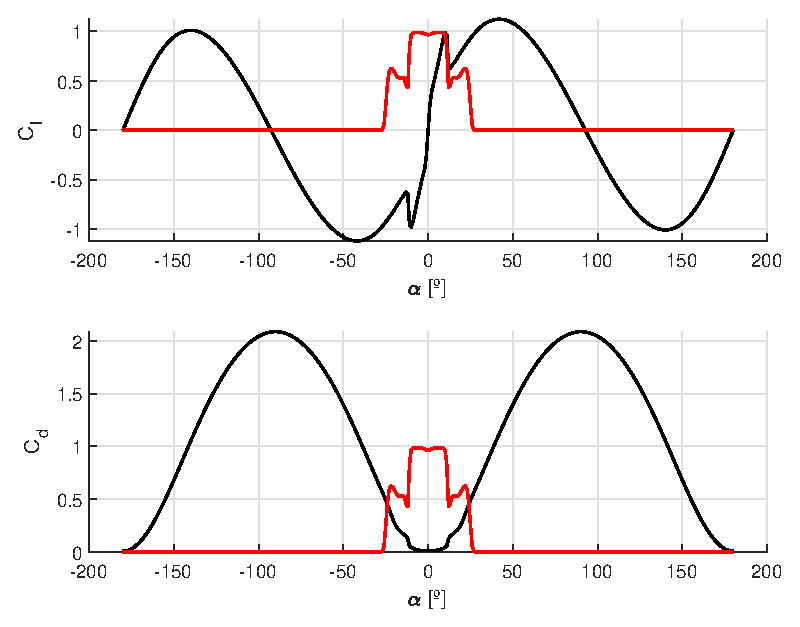
\includegraphics[width=\textwidth]{Figures/background/aero/aero_model_1e5.eps}
		\caption[NACA 0012 airfoil aerodynamic coefficients for $Re=10^5$ determined with Neural foil with confidence level]{NACA 0012 airfoil aerodynamic coefficients (in black) for $Re=10^5$determined with Neural foil with confidence level (in red)}
		\label{fig:aero_model_1e5}
	\end{minipage}
    \hfill
    \begin{minipage}{0.3\textwidth}
		\centering
		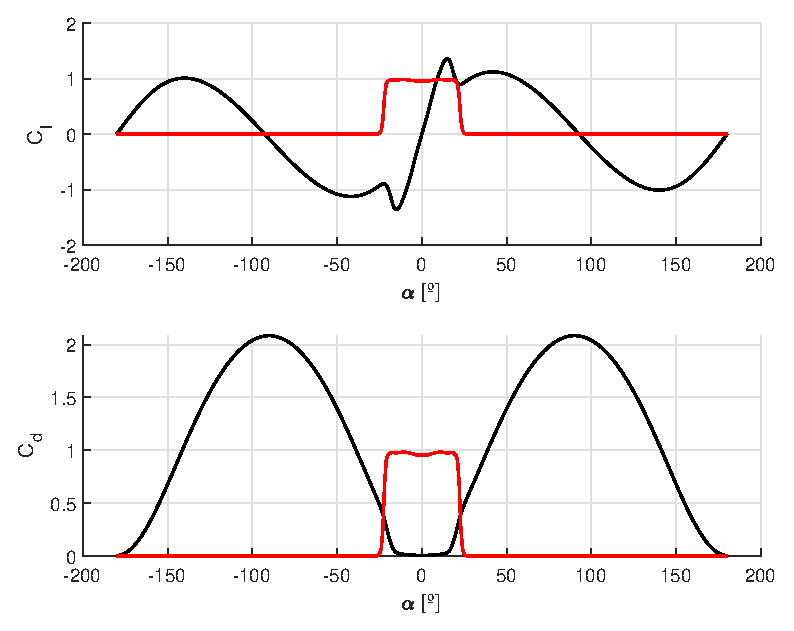
\includegraphics[width=\textwidth]{Figures/background/aero/aero_model_1e6.eps}
		\caption[NACA 0012 airfoil aerodynamic coefficients for $Re=10^6$ determined with Neural foil with confidence level]{NACA 0012 airfoil aerodynamic coefficients  (in black) for $Re=10^6$ determined with Neural foil with confidence level (in red)} 
		\label{fig:aero_model_1e6}
	\end{minipage}
\end{figure}

Once the dataset of the $C_l$ vs $\alpha$ and $C_d$ vs $\alpha$ for a wide range of angles of attack, the AERODAS's coefficents can be pre-computed for the equations in Table. \ref{tab:aerodas_key_equation}. The product of this process is simple equations that used data to model functions as presented in Fig. \ref{fig:aerodas_cl_model} and Fig. \ref{fig:aerodas_cd_model}.

Hence, with the dataset the equations can be applied to any available airfoil provided in NeuralFoil and the output is presented in Fig \ref{fig:cl_naca4412} and \ref{fig:cd_naca4412}

\begin{figure}[!htb]
    \centering
	\begin{minipage}{0.49\textwidth}
		\centering
		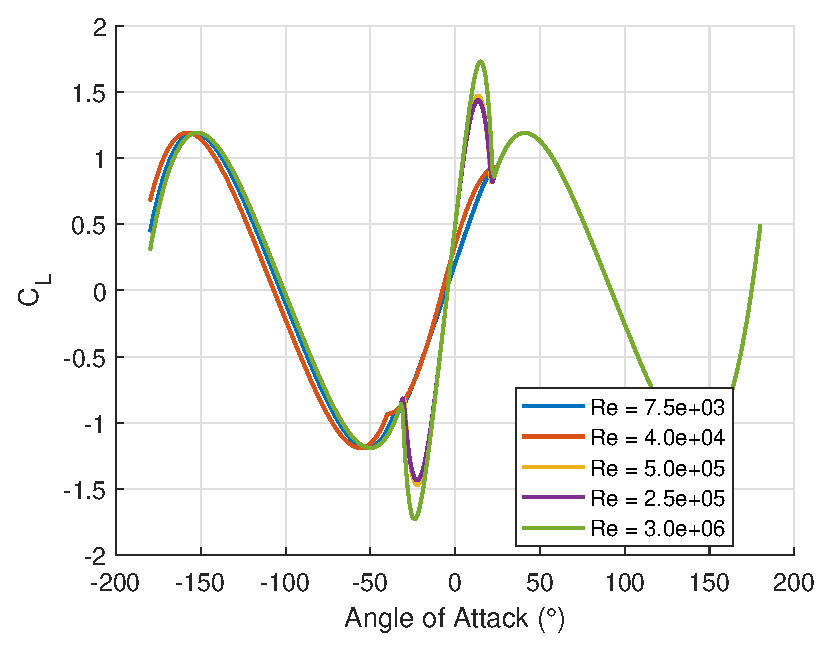
\includegraphics[width=6cm]{Figures/background/aero/cl_naca4412.eps}
		\caption{Lift coefficient computed with the presented aerodynamic model for NACA 4412 airfoil}
		\label{fig:cl_naca4412}
	\end{minipage}
    \hfill
    \begin{minipage}{0.49\textwidth}
		\centering
		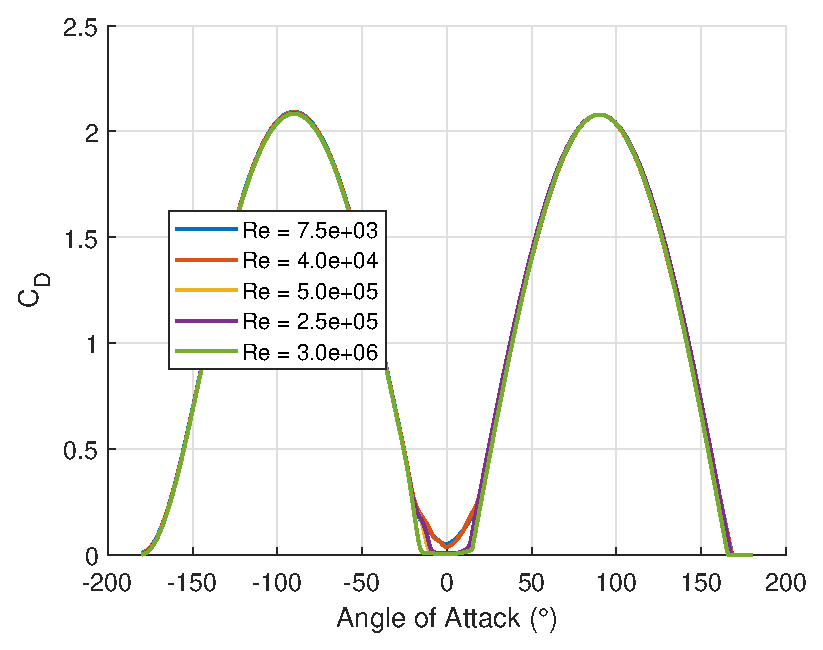
\includegraphics[width=6cm]{Figures/background/aero/cd_naca4412.eps}
		\caption{Drag coefficient computed with the presented aerodynamic model for NACA 4412 airfoil} 
		\label{fig:cd_naca4412}
	\end{minipage}
\end{figure}





%%%%%%%%%%%%%%%%%%%%%%%%%%%%%%%%%%%%%%%%%%%%%%%%%%%%%%%%%%%%%%%%%%%%%%%%
\section{Atmosphere Model}
\label{section:atmosphere_model}

The 2D aerodynamic loads, drag $\mathrm{d}D^a_n$ and lift $\mathrm{d}D^a_n$, as expressed in equations \ref{eq:drag_element} and \ref{eq:lift_element}, are directly proportional to the air density, $\rho$. Also, the atmospheric proprieties during the descent flight change with altitude, including the dynamic viscosity, $\mu$, importante to compute the Reynolds number, in equation \ref{eq:reynolds_number}. In this sense, an atmospheric model is a crucial factor when computing aerodynamic loads, as it will directly impact the values of these loads. 

On the literature there are many atmospheric models such as the \gls{isa} \cite{noauthor_iso_nodate}, \gls{nasa}'s \gls{eam} \cite{noauthor_earth_nodate} and NRLMISES00 \cite{picone_nrlmsise00_2002}. All these options seemed a good choice, but to accomplish one of  this work goals accuracy-time commitment, a critical anaylsis is necessary.

Before the analysis, for the current application, \gls{isa} model is computed using MATLAB \cite{matlab_version_2024} Aerospace Toolbox \cite{noauthor_aerospace_nodate} function \textit{atmosisa} \cite{noauthor_atmosisa_nodate} and NRLMISES00 model is computed using provided function in MATLAB \cite{matlab_version_2024} Central File Exchange \cite{noauthor_atmosphere_2025}. For the \gls{eam} a MATLAB \cite{matlab_version_2024} code was created by the author. However , not all these models compute all necessary parameteres directly, namely the dynamic viscosity, $\mu$, which further used to compute Reynolds number, $Re$. Then it was introduced the Sutherland's Law to compute the dynamic viscosity

\begin{equation}
    \mu(T) = \mu_0 \left( \frac{T_0 + S}{T + S} \right) \left( \frac{T}{T_0} \right)^{3/2}.
\end{equation}

\noindent for models EAM \cite {noauthor_earth_nodate, noauthor_atmosisa_nodate} and NRLMISES00 \cite{picone_nrlmsise00_2002, noauthor_atmosphere_2025}.

Once all the necessary code for running the different atmospheric models is completed, figures \ref{fig:atmos_models_comp_temp} and \ref{fig:atmos_models_comp_density} present a comparison of temperature and density between the three models for altitudes ranging from 0 to 100 \unit{\km}, respectively. This range was chosen to provide a clearer view of the plots for the different models. However, it is important to note that the models are not valid for all altitudes. For instance, the \gls{isa} model is valid only between sea level and the mesopause (0 to approximately 85 \unit{\km}) and the NRLMISES00 model is valid up to 1000~\unit{\km}. With \gls{eam} the height is not at limited by the model, however it only showed good agreement with the other models up to 50 \unit{\km} for the temperature profile as it can be seen in figure \ref{fig:atmos_models_comp_temp}.


\begin{figure}[!htb]
	\centering
	\begin{minipage}{0.48\textwidth}
		\centering
		\includegraphics[width=\textwidth]{Figures/background/atmos/temperature_plot.png}
		\caption{Temperature Comparison}
		\label{fig:atmos_models_comp_temp}
	\end{minipage}
	\hfill
	\begin{minipage}{0.48\textwidth}
		\centering
		\includegraphics[width=\textwidth]{Figures/background/atmos/density_plot.png}
		\caption{Density Comparison}
		\label{fig:atmos_models_comp_density}
	\end{minipage}
\end{figure}

For the density profile, all the three models shwo a good agreement with minor a relative minor error between them. However, for the temperature profile, the analysis is not so straightforward. In the lower altitudes (up to 10 km), all models exhibit a roughly linear decrease in temperature, although NRLMSISE-00 shows slight irregularities. Between 10 and 20 km, \gls{isa} displays the characteristic plateau of the tropopause, while \gls{eam} and NRLMSISE-00 present smoother transitions. Above 20 km, significant differences become apparent: NRLMSISE-00 accurately captures the sharp temperature increase in the thermosphere, reflecting its detailed physical basis, whereas \gls{isa} maintains a simplified, smoothed profile, lacking this feature. \gls{eam} diverges from \gls{isa} but does not fully replicate the extreme rise observed in NRLMSISE-00. Overall, \gls{isa} serves as a practical but simplified model, NRLMSISE-00 provides higher accuracy at extreme altitudes, and \gls{eam} strikes a balance between simplicity and realism. This comparison underscores the distinct strengths and limitations of each model in representing atmospheric temperature variations.

Further anaylsis relevante to the atmospheric models performance is presented in table \ref{tab:atmos_model_speed}, Where the execution time of diferent number of functions calls are done. From this table, it is possible to understande that the NRLMISE00 model creates a huge impact when a simulation has a low descent ratio. This is because the NRLMISE00 model is more complex and computationally expensive than the other two.

\begin{table}[!htb]
    \centering
    \begin{tabular}{
    >{\columncolor[HTML]{FFFFFF}}l 
    >{\columncolor[HTML]{FFFFFF}}r
    >{\columncolor[HTML]{FFFFFF}}r
    >{\columncolor[HTML]{FFFFFF}}r }
    \hline
    {\color[HTML]{000000} No. Function Calls} & \multicolumn{1}{r}{\cellcolor[HTML]{FFFFFF}{\color[HTML]{000000} EAM \cite{noauthor_iso_nodate}}} & \multicolumn{1}{r}{\cellcolor[HTML]{FFFFFF}{\color[HTML]{000000} ISA \cite{noauthor_earth_nodate}}} & \multicolumn{1}{r}{\cellcolor[HTML]{FFFFFF}{\color[HTML]{000000} NRLMISES00 \cite{picone_nrlmsise00_2002}}} \\ \hline
    {\color[HTML]{000000} 1}                  & {\color[HTML]{000000} 0.8 \unit{\ms}}                                                                                           & {\color[HTML]{000000} 25.1 \unit{\ms}}                                                                                        & {\color[HTML]{000000} 46.6 \unit{\ms}}                                                                                                  \\
    {\color[HTML]{000000} 10}                 & {\color[HTML]{000000} 1.0 \unit{\ms}}                                                                                           & {\color[HTML]{000000} 5.1 \unit{\ms}}                                                                                           & {\color[HTML]{000000} 25.0 \unit{\ms}}                                                                                                 \\
    {\color[HTML]{000000} 100}                & {\color[HTML]{000000} 0.1 \unit{\ms}}                                                                                           & {\color[HTML]{000000} 19.1 \unit{\ms}}                                                                                          & {\color[HTML]{000000} 173.7 \unit{\ms}}                                                                                                \\
    {\color[HTML]{000000} 1000}               & {\color[HTML]{000000} 0.4 \unit{\ms}}                                                                                           & {\color[HTML]{000000} 173.9 \unit{\ms}}                                                                                         & {\color[HTML]{000000} 1.6 \unit{\s}}                                                                                                   \\
    {\color[HTML]{000000} 10000}              & {\color[HTML]{000000} 3.0 \unit{\ms}}                                                                                           & {\color[HTML]{000000} 1.3 \unit{\s}}                                                                                             & {\color[HTML]{000000} 21.0 \unit{\s}}                                                                                                  \\
    {\color[HTML]{000000} 100000}             & {\color[HTML]{000000} 28.1 \unit{\ms}}                                                                                          & {\color[HTML]{000000} 18.1 \unit{\s}}                                                                                           & {\color[HTML]{000000} 3.7 \unit{\minute}}                                                                                                 \\ \hline
    \end{tabular}
    \caption{Computational times for different number of function calls for the three atmospheric models.}
    \label{tab:atmos_model_speed}
\end{table} 

Taking into considerantion both profile and computational anaylis clearily theres some advantages of using all the models. \gls{eam} is quite accurate and fast for low altitudes, once \gls{isa} is in accordance to the others models for altitudes until 80 \unit{\km} and realtive fast, and finally the NRLMISE00 model is the slowest computationally but provides higher varitions in certain atmosphere regions. For the final implementation, the choice of the model considered in this work, \gls{isa} is the choosen model for all the analysis presented furter in this work, once it provides quite fast computational times and a wide range of altitudes, namely the range of the DAEDALUS \cite{riegler_daedalus_2018} project used in next section to validate the model.


\section{Prandtl Tip Losses Factor}

In the context of helicopter rotor or wind turbine rotor systems, an inherent challenge arises as the blades near the tips experience a higher velocity compared to those near the hub. This speed differential introduces complications such as increased drag, heightened turbulence, and the formation of tip vortices, spiral patterns of rotating air trailing behind the rotor blade tips \cite{leishman_principles_2006}. These tip vortices signify a notable source of energy loss, which contributes to a reduction in overall system efficiency. Over the years, various strategies have been studied to mitigate this tip loss, including optimising rotor blade shapes, adjusting blade twists, and incorporating advanced aerodynamic features.

Efforts to address tip loss also involve the application of the Prandtl tip loss function \cite{leishman_principles_2006, ramdin_prandtl_nodate}. Prandtl tip loss is the decrease in aerodynamic efficiency that propeller or rotor blades undergo as they get closer to their tips as a result of following vortices that are created as they go through the air. Overall efficiency is reduced as a result of this phenomenon. Within the field of aerodynamics, the Prandtl tip loss function is a mathematical instrument that is specifically utilised to model and quantify this phenomenon \cite{leishman_principles_2006}. Its main purpose is to take into account the induced velocity caused by the tip vortices and then modify the effective inflow velocity that the blade experiences at the tip.


In the book of professor Leishman \cite{leishman_principles_2006}, the Prandtl's Tip Loss function is addressed considering two different cases: 1) no tip losses at the rotor root; 2) tip losses in tip and root of the rotor. For the first case, function which estimates a lift variation is given by equation \ref{eq:tiplossprandtl},

\begin{equation}
    F = \frac{2}{\pi} \cos^{-1}\left(\exp{\left(-f\right)}\right)
    \label{eq:tiplossprandtl}
\end{equation}

\noindent where $f$ is a function of the geometric properties of the blade and the inflow angle $\phi = \frac{\lambda (r)}{r}$

\begin{equation}
    f_{tip} = \frac{N_b}{2} \left( \frac{1-r}{r\phi}\right)
\end{equation}

Applying the the factor $F$ to the lift distribution over the blade radius, the figure \ref{fig:prandtltiploss} presents how the function varies with the number of blades and the inflow angle over the radius of the blades. From the figure \ref{fig:prandtltiploss}, is possible to see that this function does not consider the tip loss in the rotor center, as the function is the maximum value in the beginning of the rotor.

\begin{figure}[!htb]
    \centering
    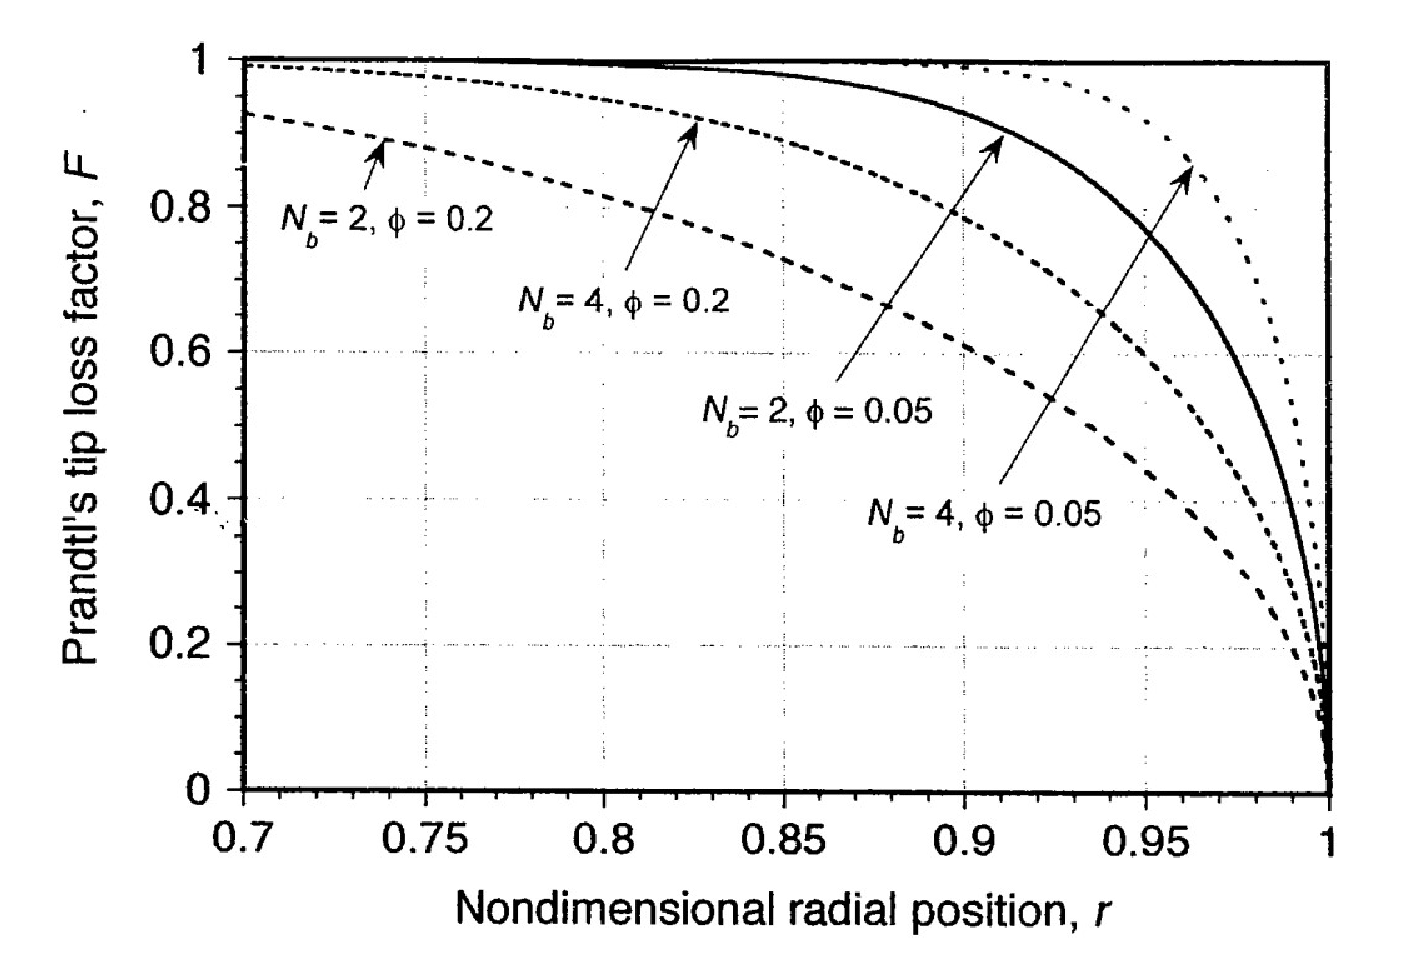
\includegraphics[width=0.5\textwidth]{Figures/background/tiplosses/prandtltiploss.eps}
    \caption[Prandtl Tip Loss function versus radial position for two- and four-bladed rotor]{Prandtl Tip Loss function versus radial position for two- and four-bladed rotor, from \cite{leishman_principles_2006}}
    \label{fig:prandtltiploss}
\end{figure}

However, this assumption is not physically correct and then the second option appears in \cite{leishman_principles_2006}. For considering the loss of tips at the root of the blade, the equation \ref{eq:tiplossesroot} is considered.

\begin{equation}
    f_{root} = \frac{N_b}{2} \left( \frac{r}{\left(1-r\right)\phi}\right)   
    \label{eq:tiplossesroot}
\end{equation}

For combining root and tip losses, the factor $f$ considered is the combinations of \ref{eq:tiplossprandtl} and \ref{eq:tiplossesroot}. The combination of root an d tip losses is presented in figure \ref{fig:fullprandtltiplossfunction}. From this figure, it is possible to conclude that, as in the tip, the root as a significant decrease in the lift force.

\begin{equation}
    F = F_{root}F_{tip}
\end{equation}

\begin{figure}[!htb]
    \centering
    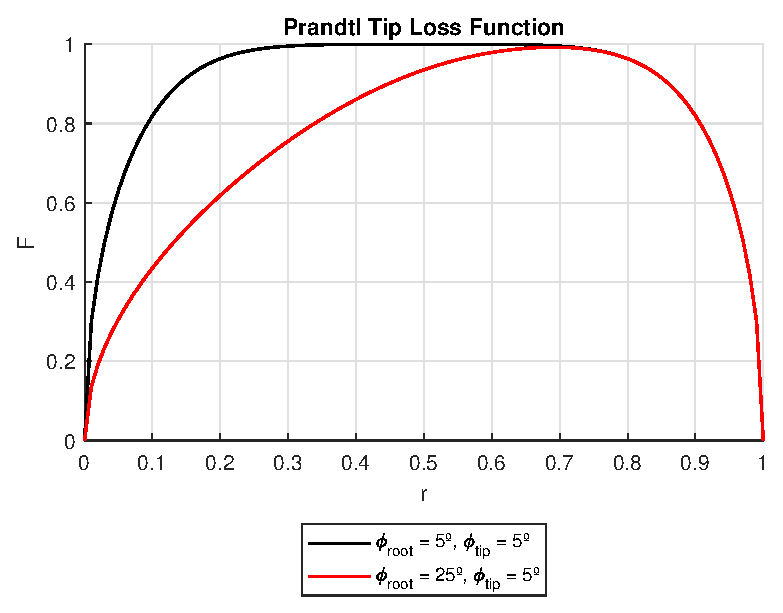
\includegraphics[width=0.5\textwidth]{Figures/background/tiplosses/prandtltiplossfunction.eps}
    \caption{Prandtl Tip Loss Function}
    \label{fig:fullprandtltiplossfunction}
\end{figure}